\documentclass{article}
\title{機械のしくみ入門 — テコからロボットまで}
\author{TeX 図書館}

\begin{document}

\section{読み方 — 機械を分解して考える 3 つの問い}

機械は黒箱に見えます。電源を入れると動く。中で何が起きているかは見えない。しかし、どんな機械でも、分解の問いは同じ 3 つです。\textbf{力はどこに入るか(入力)、どこに伝わるか(伝達)、どこで変わるか(変換)}。この 3 つの問いを機械ごとに繰り返すと、黒箱は部品の流れ図に変わります。

つまずきの原因は、ほぼ 1 つ。\textbf{原理(物理)と構造(部品)を別々に覚えようとすること}。原理だけでは実際の機械が想像できず、構造だけではなぜその形なのかが分かりません。この本では、各節を 3 段階で読みます。

\begin{itemize}
\item \textbf{【基礎】}: 支える物理の原理。高校物理やり直しの内容の再利用です。
\item \textbf{【しくみ】}: その原理を部品として組み立てる方法。
\item \textbf{【応用】}: 実際の機械・実務での使われ方。
\end{itemize}

\subsection{全 10 節の見取り図}

節の配分は次のとおりです。

\begin{enumerate}
\item 第 1 節: 読み方。3 つの問いと、本の使い方。
\item 第 2〜3 節: 力の伝達。テコ・歯車・軸・軸受。
\item 第 4〜5 節: エネルギーの変換。モーターと発電機、エンジン。
\item 第 6〜7 節: 流体と熱。ポンプ・タービン、冷蔵庫とエアコン。
\item 第 8〜9 節: 総合演習。自動車を分解する、制御される機械。
\item 第 10 節: まとめと次の一歩。
\end{enumerate}

各節の終わりには\textbf{解答の指針}を置きます。まず自力で 5 分考えてから、その欄を開いてください。

\begin{quote}
\textbf{【注意】}\ 機械の説明で最も多い誤解は「力が機械の中で消えたり増えたりする」という考えです。エネルギーは保存されます(高校物理やり直し、エネルギーの節)。機械は力を増減できても、\textbf{仕事の総量は増やせません}。力を半分にすると、距離が倍になる。このトレードオフが、すべての機械の共通項です。
\end{quote}

\textbf{解答の指針:}\ 機械の問題では、(1) 入力は何か(力・電気・熱・流れ)、(2) 途中の部品で何に変わり、何が伝わるか、(3) 出力は何か、を日本語で 1 行ずつ書く。分からない機械でも、この 3 行が書ければ、使う道具(第 2〜9 節)が決まります。逆に、3 行が書けない機械は、どこかの段階の知識が抜けているサインです。

\section{力の伝達の基礎 — テコ、滑車、歯車}

\subsection{【基礎】テコの原理とモーメント}

棒の支点から距離 \( d \) のところに力 \( F \) を加えると、棒は回ろうとします。この回ろうとする強さを\textbf{モーメント(トルク)}と呼び、\( F \times d \) で表します。単位は N・m(ニュートンメートル)。

\[ M = F \times d \]

テコの原理は、この式の直接的な帰結です。支点から遠い側に大きい距離で小さい力を加えれば、支点に近い側で小さい距離に大きい力が生まれます。\textbf{力は増やせるが、モーメント(力 × 距離)は保存される}。小さい力で動かすには、遠い側を大きく動かす必要があります。第 1 節の注意のトレードオフの最も単純な形です。

\subsection{【しくみ】滑車と歯車}

\textbf{滑車}は、テコを回転形にした道具です。\textbf{定滑車}は向きを変えるだけで力は変わりません。\textbf{動滑車}は荷物と一緒に動くので、ロープ 2 本で荷物を支える形になり、力は半分で済む代わりに、引き込むロープの長さは 2 倍になります。組み合わせれば力はさらに減らせますが、引き込む距離は同じだけ増えます。

\textbf{歯車}は、回転の伝達と速度の変換を行う部品です。歯数 20 の歯車(小)から歯数 40 の歯車(大)へ回転を伝えると、大歯車は半分の速さで回り、トルクは 2 倍になります。\textbf{回転数とトルクが逆の関係}で交換される(歯数比で決まる)のが、歯車の本質です。モーメントの話を回転でそのまま使っている形です。

\begin{figure}
\centering
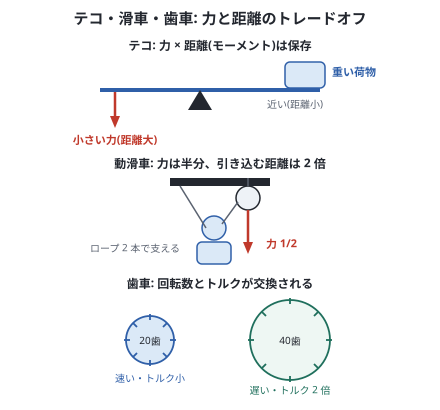
\includegraphics[width=0.9\textwidth]{figures/lever-gear.svg}
\caption{テコ・滑車・歯車: 力と距離(回転数)のトレードオフ}
\end{figure}

\subsection{【応用】自転車の変速機}

自転車は、この節の道具の総合演習です。ペダルのクランク(テコ)で足の力をトルクに変え、チェーンで後輪のスプロケット(歯車)へ伝えます。\textbf{重いギア}はスプロケットが大きく、1 回転あたり進む距離は長いがトルクは軽い。\textbf{軽いギア}はその逆。坂道で軽いギアにするのは「力は半分、回転数は 2 倍」のトレードオフを選んでいるだけで、物理的には「テコの長さを変えている」のと同じです。

\begin{quote}
\textbf{【注意】}\ 「機械で力を増やせるなら、増やした分だけ楽になる」と考えるのが最大の誤解です。仕事(力 × 距離)は保存されます。むしろ実際の機械では摩擦が仕事を熱に変えるので、\textbf{入力の仕事より出力の仕事は必ず減ります}。効率 100 パーセントの機械は存在しません。
\end{quote}

\textbf{解答の指針:}\ 力の伝達の問題では、(1) 入力側の力と距離(または回転数とトルク)を書く、(2) 伝達部の歯数比・ロープの本数を確認する、(3) 出力側の力と距離を書いて、力 × 距離が保存(実際は摩擦分だけ減少)しているか確かめる。効率を問われたら、出力 ÷ 入力です。トレードオフを明示できるかが理解の目安です。

\section{回転を支える部品 — 軸、軸受、ベルト、チェーン}

\subsection{【基礎】回転の運動}

回転する物体には、直線運動の慣性に対応する\textbf{慣性モーメント}があります。重い部分が軸から遠いほど回しにくく、回した分だけ止めにくい。この性質が、フライホイール(はずみ車)の原理です。\textbf{回転のエネルギーを一時的に溜めて、供給のむらを平滑化する}部品として、エンジンやプレス機に組み込まれています。

回転を変える要素は 3 つに整理できます。\textbf{軸}(回転を運ぶ棒)、\textbf{軸受}(回転を滑らかに支える)、\textbf{伝達要素}(ベルト・チェーン・歯車で回転を別の軸へ渡す)。機械の中身の大半は、この 3 つの組み合わせです。

\subsection{【しくみ】軸受と伝達の仕組み}

\textbf{軸受(ベアリング)}は、軸が摩擦なく回るための部品です。転がり軸受は、軸と外輪の間に小球を転がし、滑り摩擦を転がり摩擦に置き換えます。転がり摩擦は滑り摩擦よりずっと小さいので、少ない力で回り続けます。摩擦を減らすことは、第 2 節の注意(仕事の損失)への直接的な対処です。

\textbf{ベルトとチェーン}は、離れた 2 つの軸の間で回転を伝えます。ベルトは静かに伝えるが、強い力では滑る(古い回転体のスリップ)。チェーンは滑らず強いが、油差しと音が要る。\textbf{滑るか、鳴るか}のトレードオフは、伝達の設計の基本の選択肢です。自転車のチェーンと、洗濯機やパワーツールのベルトが、それぞれの解です。

\subsection{【応用】身のまわりと工場}

ドアの蝶番(軸受の極端な小型版)、回転寿司のレール(ベルト伝達)、自転車のクランク(軸 + 軸受 + チェーン)、電動ドライバー(モーター + 歯車列)。すべての回転機械は、この節の部品の組み合わせです。分解の問いを当てはめると、「回転はどの軸からどの軸へ、何で伝わっているか」が必ず書けます。

\begin{quote}
\textbf{【注意】}\ 回転部品の破損原因の多くは過度の摩擦と熱です。油は摩擦を減らすと同時に熱を運び出します。「油が切れる」ことが機械の死に直結するのは、摩擦と熱の管理が伝達の生命線だからです。
\end{quote}

\textbf{解答の指針:}\ 部品の問題では、(1) どの軸が回るか、(2) どこで支えられ、どこで伝わるか、(3) 摩擦と熱がどこに出るか、を書く。故障の問題では、「摩擦・熱・振動」の 3 つのうちどれが原因かを疑い、軸受・油・伝達の緩みの順で確認する手順を書きます。

\section{モーターと発電機 — 電気と回転の往復}

\subsection{【基礎】電磁石と力}

電線に電流を流すと磁場が生まれます(電磁気の基本)。コイルに巻けば磁場が集まり、鉄心に入れれば強い\textbf{電磁石}になります。さらに、磁場の中で電流を流す導体には力が働きます。この\textbf{「磁場の中の電流に力が働く」}のが、モーターのすべての原理です。

\[ F = BIL \]

磁場 \( B \) の中に、長さ \( L \) の導体で電流 \( I \) を流すと、力 \( F \) が働きます(向きは 3 者すべてに垂直)。

\subsection{【しくみ】コイルを回す}

モーターの構造は単純です。磁石の間にコイルを置き、電流を流すとコイルに力が働いて半回転しようとします。\textbf{整流子}(回転に合わせて電流の向きを切り替える部品)があれば、半回転するごとに電流が反転し、同じ向きの力が続いて回り続けます。

\textbf{発電機}は、この逆向きです。コイルを磁場の中で回すと、コイルを貫く磁場の量が変わり、電気が生まれます(電磁誘導)。モーターと発電機は\textbf{同じ構造で、電気と回転のどちらを入れるかが違うだけ}です。モーターに手で回軸を回せば発電機になり、発電機に電気を入れても回ります。

\begin{figure}
\centering
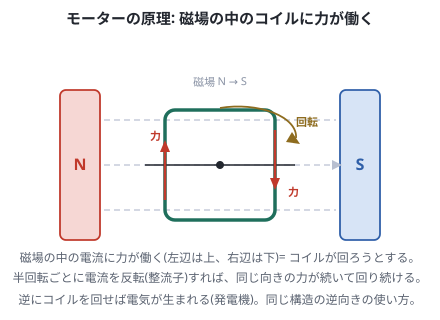
\includegraphics[width=0.9\textwidth]{figures/motor-principle.svg}
\caption{モーターの原理: 磁場の中のコイルに力が働き、回転する}
\end{figure}

\subsection{【応用】家電から発電所、電気自動車まで}

小型モーターは家電のどこにでもいます(扇風機、洗濯機、ドライヤー、歯ブラシ)。発電所も本質は発電機で、\textbf{何で回すか}(水車・蒸気タービン・風)が発電方式の名前になっています。\textbf{電気自動車}は、モーター特有の性質を端的に示す例です。回り始めから最大トルクが出る(エンジンは回転数が上がらないと力が出ない)ので、変速機が不要で静かで、加速が速い。

\begin{quote}
\textbf{【注意】}\ モーターも発電機も、電気と回転のエネルギー交換で損失(主に熱)が発生します。モーターが熱くなるのは、電気抵抗と磁気損失が仕事を熱に変えているからです。性能の議論は「効率」で行い、宣伝文句の「強力」ではなく出力と損失の両方を見ます。
\end{quote}

\textbf{解答の指針:}\ モーターの問題では、(1) 磁場の向き、電流の向き、力の向きの 3 者を絵で書く(2 者が決まれば 3 者は決まる)、(2) 回転し続けるには何が必要か(電流の反転)を確認する、(3) 発電機なら回転が電気を生む方向に話を逆にする。3 者の向きの絵が描けるかどうかが、この分野の理解の全てです。

\section{エンジン — 熱を運動に変える}

\subsection{【基礎】熱膨張と圧力}

気体は熱せられると膨張します(高校物理やり直し、粒子モデルの節)。膨張する気体がピストンを押せば、\textbf{熱のエネルギーが運動のエネルギーに変わる}。エンジンは、この変換を繰り返し行う装置です。燃料を燃やして高温高圧の気体を作り、その膨張で機械を動かします。

\subsection{【しくみ】4 ストロークのサイクル}

自動車のガソリンエンジンは、4 つの工程を 1 サイクルとして繰り返します。

\begin{enumerate}
\item \textbf{吸入}: ピストンが下がり、燃料と空気の混合気を吸い込む。
\item \textbf{圧縮}: ピストンが上がり、混合気を小さな体積に押し込む。
\item \textbf{燃焼}: スパークプラグで点火し、急激な膨張でピストンを押し下げる。\textbf{ここだけが仕事を出す工程}です。
\item \textbf{排気}: 燃え殻を外へ出す。
\end{enumerate}

ピストンの上下運動は、\textbf{クランク機構}で回転運動に変換されます(自転車のペダルと同じ変換)。4 つの工程のうち、実際に力を出すのは燃焼の 1 工程だけ、という事実がエンジン設計の中心であり、フライホイール(第 3 節)が残りの 3 工程を持ち回る仕組みになっています。

\subsection{【応用】効率と電動化}

エンジンの効率には理論上の上限があります(熱力学の制約で、燃焼の熱の一部は必ず排気と冷却で捨てられる)。ガソリンエンジンの実効効率は 3〜4 割程度で、残りは熱として逃げています。\textbf{ディーゼルエンジン}は圧縮比を高くできる分、効率が良い代わりに構造が丈夫(高圧に耐える)で振動が大きい。\textbf{電気自動車}は、モーターの効率が 9 割近くある点と、止まっているときはエネルギーを使わない点で、エンジンと構造的に違います。この比較は「効率」の数値で行い、感覚ではなく数値で判断する習慣をつけてください。

\begin{quote}
\textbf{【注意】}\ 「エンジンは燃料を燃やす機械」は正しいですが、「燃料のエネルギーが全部運動になる」は誤りです。3 割以上が熱として捨てられる、という事実を前提にして、エンジンの設計(冷却・排気・ターボ)を読み解くのが正しい姿勢です。
\end{quote}

\textbf{解答の指針:}\ エンジンの問題では、(1) 4 工程のどの工程か(または全体の流れか)を書き、(2) 仕事を出す工程が 1 つだけであることを確認する、(3) 効率の議論では入力(燃料)と出力(運動)と損失(熱)の 3 本立てで書く。クランク機構は上下運動と回転の変換だと、第 2 節のテコの話とつなげて説明できるかが理解の目安です。

\section{ポンプ、圧縮機、タービン — 流体を扱う機械}

\subsection{【基礎】圧力と流れ}

流体(液体と気体)は、圧力の高いところから低いところへ流れます。\textbf{ポンプ}はこの流れを逆に作る機械です(低いところから汲み上げる)。圧力の単位は Pa(パスカル)で、1 気圧は約 101 kPa です。水 10 m の高さは約 1 気圧に相当します(水柱 10 m で 98 kPa)。

\subsection{【しくみ】2 つの方式}

ポンプには 2 つの方式があります。\textbf{容積式}は、室を広げて吸い込み、狭めて押し出す方式で、手動ポンプや高圧用に使います(確実に押し出すが脈動する)。\textbf{遠心式}は、羽根(インペラ)を高速で回し、遠心力で流体を外へ飛ばす方式で、大量の流体を連続的に送れます(水道・ポンプの主流)。

\textbf{圧縮機}は気体用のポンプです。気体は体積を狭めると圧力が上がる(同じ分子数を小さな室に押し込む)ので、圧縮機は圧力の高い気体を作ります。エアコンの室外機の中身は圧縮機です(第 7 節)。\textbf{タービン}は、ポンプの逆で、\textbf{流れる流体で羽根を回す}機械です。水力発電の水車、蒸気タービン、風車。ジェットエンジンは「圧縮機で空気を押し込み、燃焼し、タービンで圧縮機を回す」組み合わせです。

\subsection{【応用】水道からジェットエンジンまで}

水道は浄水場のポンプが圧力を作り、高低差と管の抵抗との釣り合いで家まで水を届けます。給湯や空調の配管も同じ力の流れです。\textbf{ジェットエンジン}は、この節と第 5 節の総合演習です。ファンで空気を吸い込み、圧縮機で圧力を上げ、燃焼室で燃料を燃やし、高温のガスがタービンを回して(圧縮機を駆動して)残りをジェットとして後方へ噴く。圧縮機とタービンが同軸でつながっている、という構造を覚えると、ジェットエンジンの断面図が読めるようになります。

\begin{quote}
\textbf{【注意】}\ ポンプが汲み上げられる高さには理論上の限界があります(大気圧が押し上げられる水柱は約 10 m)。 suction(吸い上げ)は大気圧との差で押し上げるだけなので、それ以上の高さは、ポンプを上に置くか(押し上げ方式)、多段にします。配管設計の基本の制約です。
\end{quote}

\textbf{解答の指針:}\ 流体機械の問題では、(1) 扱うのは液体か気体か、(2) 圧力を上げるのか、回転を取り出すのか(ポンプかタービンか)、(3) 容積式か遠心式か、を書く。ジェットエンジンのような複合機械は、空気の流れに沿って部品を順に並べ、各段で圧力と温度がどう変わるかを図にします。

\section{熱を運ぶ機械 — 冷蔵庫とエアコン}

\subsection{【基礎】気化熱と圧力で決まる沸点}

液体が気化するとき、周囲から大量の熱を奪います(気化熱)。アルコールを手に付けると冷たいのはこのためです。そして\textbf{沸点は圧力で変わる}という性質が鍵です。圧力を下げれば低い温度で沸騰し、圧力を上げれば高い温度で沸騰します。圧力鍋が高温になるのも同じ原理です。

\subsection{【しくみ】冷媒サイクルの 4 工程}

冷蔵庫とエアコンは、\textbf{熱を冷たい側から暖かい側へ運ぶ}機械(ヒートポンプ)です。自然には熱は高温から低温へ流れる(第 1 節のエネルギーの話)ので、逆流させるには仕事(電力)が必要です。冷媒という物質を循環させて熱を運びます。

\begin{enumerate}
\item \textbf{圧縮}: 圧縮機で冷媒ガスを高圧にする(沸点が上がる)。
\item \textbf{凝縮}: 高圧のガスが外側(暖かい側)で熱を出して液体になる。
\item \textbf{膨張}: 膨張弁で急に圧力を下げる(沸点が下がる)。
\item \textbf{蒸発}: 低圧の液体が内側(冷たい側)で沸騰し、周囲から熱を奪って気化する。
\end{enumerate}

\textbf{冷蔵庫とエアコンは同じ構造}です。違いはどちら側を室内に置くかだけ。冷蔵庫は蒸発器を庫内に、エアコンは蒸発器を室内に置きます(冷房時)。この対応が分かると、「エアコンで冷やしながら室外機が熱い」理由が自明になります。\textbf{奪った熱と圧縮の仕事の熱を、全部外へ出しているからです}。

\begin{figure}
\centering
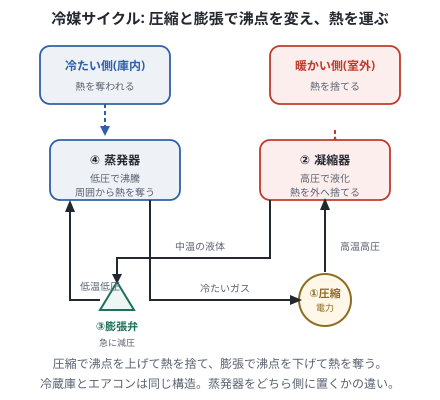
\includegraphics[width=0.9\textwidth]{figures/refrigeration-cycle.svg}
\caption{冷媒サイクル: 圧縮と膨張で沸点を変え、熱を運ぶ}
\end{figure}

\subsection{【応用】効率(COP)と暖房}

ヒートポンプの効率は\textbf{COP}(成績係数)で測ります。COP 3 とは、電力 1 で熱 3 を移動できるという意味です。移動ですから、\textbf{1 より大きい}のが普通です(エンジンは 1 未満)。暖房として使うときも同じサイクルを逆に回すだけで(冷媒の流れを切り替える)、効率の良い暖房になります。電気ストーブ(COP 1)とエアコン暖房(COP 3 以上)の違いは、\textbf{熱を作るか、熱を運ぶか}の違いです。

\begin{quote}
\textbf{【注意】}\ 「冷蔵庫は熱を消している」ではありません。\textbf{熱を庫内から外へ運んでいる}だけです。扉を開けっ放しにして部屋を冷やそうとしても、庫内から奪った熱とモーターの熱が全部部屋に戻るので、部屋はむしろ暖かくなります。エネルギーの収支を書けば即座に分かる、定番の思考実験です。
\end{quote}

\textbf{解答の指針:}\ 熱機械の問題では、(1) 熱の移動の方向(自然の流れと逆方向か)を確認する、(2) 4 工程を冷媒の状態(高温高圧 → 液化 → 低圧 → 気化)とともに書く、(3) COP = 移動した熱 ÷ 電力 で効率を評価する。扉開放の問題のような思考実験は、部屋全体の熱収支を 1 枚の図に書けば解けます。

\section{自動車を分解する — 動力伝達の総合演習}

\subsection{【基礎】力の流れを 1 本にたどる}

自動車は、この本の前半の道具の総合演習です。力の流れは 1 本です。\textbf{エンジン(熱 → 回転) → 変速機(トルクと回転数の変換) → 差動歯車(左右の輪へ分配) → タイヤ(回転 → 前進)}。各段で、第 2 節の歯車と第 5 節のエンジンの道具が使われています。

\subsection{【しくみ】変速機と差動、ブレーキ}

\textbf{変速機}(トランスミッション)は、エンジンの特性と走行条件を合わせる装置です。エンジンは回転数が適切な範囲でしか効率よく力を出しません。発進時は大きなトルク(軽いギア)、高速走行は小さなトルクで長く回す(重いギア)。自転車の変速(第 2 節)と同じトレードオフを、歯車列で自動化したものです。

\textbf{差動歯車(デフ)}は、コーナーで左右のタイヤの回転数が違うことを許す装置です。曲がるとき内側のタイヤは回る距離が短い。左右を固くつなぐと、どちらかが滑ります。差動は「平均を取りつつ差を許す」歯車の組み合わせで、この矛盾を解決します。

\textbf{ブレーキ}は、運動エネルギーを熱に変換する装置です(エネルギー保存の直接的な応用)。ディスクブレーキは、回転する円盤をパッドで挟んで摩擦熱にします。回生ブレーキ(電気自動車)は、モーターを発電機として使い、運動エネルギーを電気として回収します。第 4 節の「モーターと発電機は同じ構造」の直接的な応用です。

\subsection{【応用】効率と安全の設計}

自動車の燃費改善は、この本の道具の言い換えです。摩擦の削減(第 3 節)、エンジン効率(第 5 節)、車重の軽減(運動エネルギーの削減)、回生ブレーキ(エネルギーの回収)。安全設計は「衝突のエネルギーをどこで吸収するか」の設計で、クランプルゾーン(潰れる領域)が運動エネルギーを変形の仕事に変換します(高校物理やり直し、仕事の節)。

\begin{quote}
\textbf{【注意】}\ 自動車の「馬力」と「トルク」を混同する議論は定番の誤解です。トルクは回す力、馬力(パワー)は単位時間あたりの仕事です。両者は回転数で結ばれます。加速の実感は主にパワーと車重の比で決まる、と数値で押さえておくと議論が整理されます。
\end{quote}

\textbf{解答の指針:}\ 自動車の問題では、(1) 力の流れを 1 本の矢印で書く(エンジン → 変速 → 差動 → タイヤ)、(2) 各段の変換(トルク・回転数・エネルギーの形)を書き添える、(3) 問われた部品がどの段で何をしているかを特定する。回生ブレーキの問題は、エネルギーの流れ(運動 → 電気 → 電池)で書けば解けます。

\section{制御される機械 — エレベーターとロボット}

\subsection{【基礎】釣り合いと安全}

\textbf{エレベーター}の核心は、\textbf{釣り合いおもり}(カウンターウェイト)です。かごの重さとほぼ同じ重りをロープの反対側に下げておくと、モーターは「乗客の重さ」だけを持ち上げればよくなります。力のトレードオフ(第 2 節)ではなく、\textbf{重さを相殺して無駄を消す}発想です。人が乗っていない状態で、かごと重りが釣り合えば、モーターの仕事は最小になります。

安全装置は多重化されています。調速機(速度を監視)、非常ブレーキ、緩衝器(最下層の衝撃吸収)。\textbf{制御系の故障を想定して、物理的な安全装置を別に置く}のが機械の安全設計の原則です。

\subsection{【しくみ】フィードバック制御のループ}

\textbf{ロボット}を動かしているのは、\textbf{フィードバック制御}です。ループの構造は 4 つです。

\begin{enumerate}
\item \textbf{目標}: 「腕を 30 度まで動かす」のような命令。
\item \textbf{センサー}: 今の状態を測る(角度、速度、力、位置)。
\item \textbf{比較}: 目標と現在の差(誤差)を計算する。
\item \textbf{操作}: 誤差が小さくなる方向にモーターを動かす。
\end{enumerate}

このループを高速で回し続けることで、ロボットは「目標 → 行動 → 確認 → 修正」を自動で繰り返します。\textbf{サーボモーター}は、このループを内蔵したモーターで、指定の角度まで自力で回って止まる部品です。ロボットアームは、サーボモーターを関節ごとに並べたものと読めます。

\begin{figure}
\centering
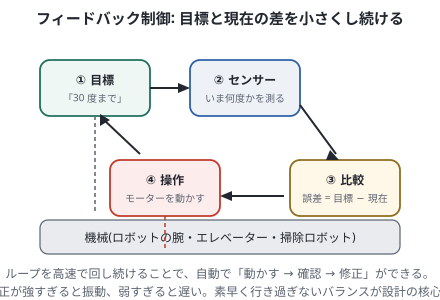
\includegraphics[width=0.9\textwidth]{figures/control-loop.svg}
\caption{フィードバック制御: 目標と現在の差を小さくし続けるループ}
\end{figure}

\subsection{【応用】センサーの種類と設計の感覚}

センサーの代表は、\textbf{位置}(エンコーダ)、\textbf{力}(ひずみゲージ)、\textbf{光}(カメラ、LiDAR)、\textbf{温度・圧力}です。センサーの質が制御の質を決めます(測れないものは制御できません)。掃除ロボットは、位置センサーと衝突センサーでループを回している、と読めます。人間の運動も同じ構造(目標 → 筋の力 → 体の感覚 → 修正)で、心理学入門の知覚・運動の話とつながります。

\begin{quote}
\textbf{【注意】}\ フィードバック制御には落とし穴があります。修正が強すぎると行き過ぎて振動し(オーバーシュートの繰り返し)、弱すぎると目標に届くまで時間がかかります。\textbf{素早く、行き過ぎない}バランスを取るのが制御設計の核心で、実際の設計は数値の調整の世界です。
\end{quote}

\textbf{解答の指針:}\ 制御の問題では、(1) 目標・センサー・比較・操作の 4 つがどこにあるかを書く、(2) 誤差がどのように減るかを 1 行で説明する、(3) 安全の問題では、制御の故障とは別の物理的安全装置(ブレーキ・緩衝器)を探す。釣り合いおもりの問題は、重さの収支(上げる物 − 釣り合わせる物 = モーターの負担)で書けば解けます。

\section{まとめと次の一歩}

9 節を振り返ります。機械を見る目は、3 つの問いと 5 つの道具です。

\begin{itemize}
\item \textbf{3 つの問い}: 力はどこに入り、どこに伝わり、どこで変わるか。
\item \textbf{トレードオフ}: 力と距離(回転数)は交換でき、仕事は保存される。
\item \textbf{変換の道具}: テコ・歯車(力)、モーター・発電機(電気と回転)、ポンプ・タービン(流体)、ヒートポンプ(熱)。
\item \textbf{効率}: 出力 ÷ 入力。損失は主に熱。
\item \textbf{制御}: 目標と現在の差を小さくし続けるループ。
\end{itemize}

機械の学習で一番効くのは、\textbf{身のまわりの機械を 1 台分解して問いを書くこと}です(実際に分解しなくても、絵で構いません)。扇風機でも自転車でもよい。読んだ節の道具で 3 つの問いに答え、力の流れ図を 1 枚描いてください。機械は「分かった気」になりやすい分野ですが、流れ図が描けるかどうかで理解の質が全く変わります。

次の一歩としては、この本の先は次のような本へつながります。

\begin{itemize}
\item 力とエネルギーの物理をやり直す → \textbf{高校物理やり直し}(力・エネルギー・電磁気の節)
\item 電気と磁場の計算の先 → \textbf{大学数学入門}(ベクトルが磁場と力の計算を支えます)
\item 制御とセンサーのデータの読み方 → \textbf{統計学入門}(センサーの誤差とノイズの世界)
\item 熱のやり取りの根拠 → \textbf{高校化学やり直し}(粒子モデルと状態変化)
\end{itemize}

機械は、物理の原理が部品になったものです。3 つの問いを持って機械を見ると、黒箱がはじめて透明になります。まずは自転車の力の流れを 1 枚の図に描くことから始めてください。

\end{document}
